%%%%%%%%%%%%%%%%%%%%%%%%%%%%%%%%%%%%%%%%%%%%%%%%%%%%%%%%%%%%%%%%%%%%%%%%
%Desarrollo de un juego para Nintendo DS | Trabajo de Fin de Grado
% Escuela Politécnica Superior de la Universidad de Alicante
% Realizado por: Carla Maciá Díez
% Contacto: carlamd1997@hotmail.com / cmd23@alu.ua.es
%%%%%%%%%%%%%%%%%%%%%%%%%%%%%%%%%%%%%%%%%%%%%%%%%%%%%%%%%%%%%%%%%%%%%%%%

\chapter{Anexo I - Detalles técnicos de Nintendo DS}
\label{anexo}

\section{Procesadores}

Como hemos mencionado la Nintendo DS posee dos unidades de procesamiento que realizan tareas diferentes y específicas. Vamos a profundizar continuación un poco en dichos procesadores para conocer algunos datos técnicos sobre ellos y los trabajos que llevarán a cabo en cualquier juego que se ejecute en la NDS.

\vspace{1cm}

\subsection{ARM9}

Su nombre completo es \textbf{ARM946E-S} y pertenece a la familia de procesadores de \textbf{32 bits}, con una arquitectura \textbf{RISC}\footnote{RISC: del inglés \textit{Reduced Instruction Set Computer}, es un tipo de diseño de procesadores que tiene como objetivo reducir los accesos a memoria y con ello hacer más eficiente la ejecución de instrucciones.}, conocida como ARM9. Aunque oficialmente se conozca ARM9 como el nombre que se le da a esta familia de procesadores, nosotros durante este documento usaremos ese término para referirnos al procesador ARM946E-S en concreto.

\vspace{0.5cm}

Este procesador es capaz de trabajar a una frecuencia de \textbf{66MHz}, haciéndolo el más potente de los dos procesadores de la NDS. Además, su diseño está basado en la \textbf{arquitectura Harvard} para el acceso a memoria, lo cual quiere decir que la memoria está separada en memoria de datos y memoria de instrucciones, permitiéndole acceder simultáneamente a ambas y mejorando su rendimiento a cambio de una mayor complejidad.

\vspace{0.5cm}

Por otro lado, el ARM9 usa un \textit{pipeline}\footnote{En informática, un \textit{pipeline} o tubería se refiere a una lista de procesos consecutivos donde la entrada de uno es la salida del que le precede.} de \textbf{5 pasos}. Primero, obtiene la instrucción a realizar de una cola de prioridad, después la decodifica, seguidamente la ejecuta, accede a datos en memoria (si la instrucción lo requiere), y finalmente vuelve a escribir en los registros de las instrucciones.

\vspace{0.5cm}

 \begin{figure}[htbp]
\centering
  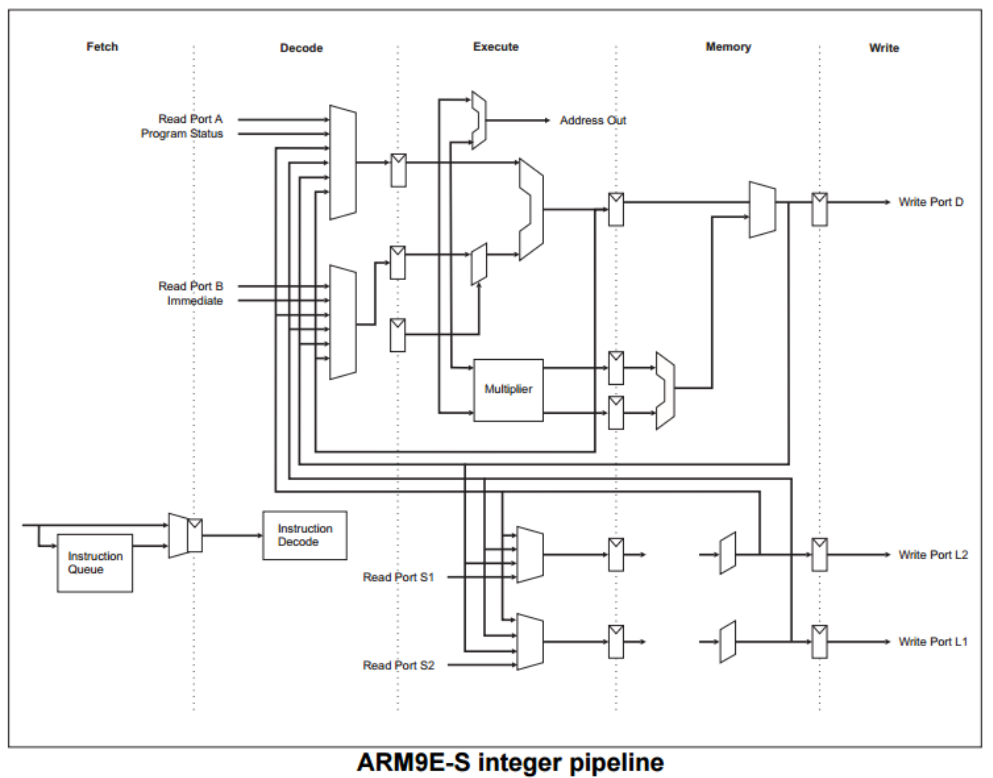
\includegraphics[width=0.5\textwidth]{archivos/arm9pipeline.png}
  \caption{Representación gráfica de la tubería de procesos del ARM9}
\textbf{Fuente:} \href{http://meseec.ce.rit.edu/551-projects/fall2015/3-1.pdf}{Thomas Farrell y Connor Petilli}
  \label{fig:arm9pipeline}
\end{figure}

\vspace{0.5cm}

Por último debemos comentar las tareas de este procesador. En general, se encarga del \textbf{90\% de la ejecución} de los juegos de NDS, tanto toda la lógica, algoritmos, IA e incluso la parte gráfica. Sin embargo, en la ejecución de \textbf{juegos de GBA no se usa}, dejándole esa tarea al ARM7.

\vspace{1cm}

\begin{comment}
\begin{table}[htbp]
\centering
\begin{tabular}{lll}
\hline
\multicolumn{1}{|l|}{00000000h} & \multicolumn{1}{l|}{Instrucciones TCM}                    & \multicolumn{1}{l|}{32KB (inamovible, puede reflejarse en 1000000h)} \\ \hline
\multicolumn{1}{|l|}{0xxxx000h} & \multicolumn{1}{l|}{Memoria TCM}                          & \multicolumn{1}{l|}{16KB (movible)}                                  \\ \hline
\multicolumn{1}{|l|}{02000000h} & \multicolumn{1}{l|}{Memoria principal}                    & \multicolumn{1}{l|}{4MB}                                             \\ \hline
\multicolumn{1}{|l|}{03000000h} & \multicolumn{1}{l|}{WRAM Compartida}                      & \multicolumn{1}{l|}{0KB, 16KB, o 32KB pueden ser asignados al ARM9}  \\ \hline
\multicolumn{1}{|l|}{04000000h} & \multicolumn{1}{l|}{Puertos de comunicación del ARM9}     & \multicolumn{1}{l|}{}                                                \\ \hline
\multicolumn{1}{|l|}{05000000h} & \multicolumn{1}{l|}{Memoria para paletas (ambos motores)} & \multicolumn{1}{l|}{2KB}                                             \\ \hline
\multicolumn{1}{|l|}{06000000h} & \multicolumn{1}{l|}{VRAM - Motor A (fondos)}              & \multicolumn{1}{l|}{max 512KB}                                       \\ \hline
\multicolumn{1}{|l|}{06200000h} & \multicolumn{1}{l|}{VRAM - Motor B (fondos)}              & \multicolumn{1}{l|}{max 128KB}                                       \\ \hline
\multicolumn{1}{|l|}{06400000h} & \multicolumn{1}{l|}{VRAM - Motor A (sprites)}             & \multicolumn{1}{l|}{max 256KB}                                       \\ \hline
\multicolumn{1}{|l|}{06600000h} & \multicolumn{1}{l|}{VRAM - Motor B (sprites)}             & \multicolumn{1}{l|}{max 128KB}                                       \\ \hline
\multicolumn{1}{|l|}{06800000h} & \multicolumn{1}{l|}{VRAM - "LCDC"-allocated}              & \multicolumn{1}{l|}{max 656KB}                                       \\ \hline
\multicolumn{1}{|l|}{07000000h} & \multicolumn{1}{l|}{OAM}                                  & \multicolumn{1}{l|}{2KB}                                             \\ \hline
\multicolumn{1}{|l|}{08000000h} & \multicolumn{1}{l|}{GBA Slot ROM}                         & \multicolumn{1}{l|}{32MB}                                            \\ \hline
\multicolumn{1}{|l|}{0A000000h} & \multicolumn{1}{l|}{GBA Slot RAM}                         & \multicolumn{1}{l|}{64KB}                                            \\ \hline
\multicolumn{1}{|l|}{FFFF0000h} & \multicolumn{1}{l|}{ARM9-BIOS}                            & \multicolumn{1}{l|}{32KB, solo 3KB usados}                           \\ \hline
                                &                                                           &                                                                     
\end{tabular}
\caption{Mapa de memoria del ARM9.}
\label{table:arm9spec}
\end{table}

\end{comment}

\subsection{ARM7}

Al igual que con el ARM9, su nombre completo es \textbf{ARM7TDMI}, pero durante este documento nos referiremos a él como ARM7. Este procesador es también de la familia de procesadores ARM7, de arquitectura \textbf{RISC} de \textbf{32 bits}.

\vspace{0.5cm}

Es algo \textbf{menos potente} que el anterior, pues su velocidad es de \textbf{33MHz} en la ejecución de \textbf{juegos de NDS} y \textbf{16MHz en los de GBA}. Además, se diferencia con respecto al ARM9 en su diseño en lo referente al acceso a memoria, pues este sigue una \textbf{arquitectura de Von Neumann}. Mientras que el ARM9 separaba entre memoria de datos y memoria de instrucciones teniendo dos buses de datos distintos, el ARM7 tiene un único bus de 32 bits para estos.

\vspace{0.5cm}

Por otro lado, su \textit{pipeline} se basa únicamente en \textbf{3 pasos}, siendo la obtención de instrucciones de memoria, decodificación y ejecución de estas. No posee una memoria caché\footnote{Componente hardware que guarda datos de recurrente uso en una memoria más accesible para el procesador de modo que en futuras solicidudes de estos datos el tiempo de lectura de estos será menor.} para instrucciones o datos, pero esto se ve recompensado con una mayor velocidad en el flujo de las instrucciones.

\vspace{0.5cm}

 \begin{figure}[htbp]
\centering
  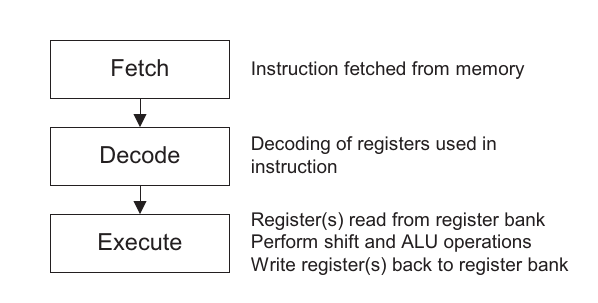
\includegraphics[width=0.5\textwidth]{archivos/arm7pipeline.png}
  \caption{Representación gráfica de la tubería de procesos del ARM7}
\textbf{Fuente:} \href{http://ww1.microchip.com/downloads/en/DeviceDoc/DDI0029G_7TDMI_R3_trm.pdf}{ARM}
  \label{fig:arm7pipeline}
\end{figure}

\vspace{0.5cm}

Por último, este procesador no juega un papel tan importante como el ARM9, pero sí realiza tareas de gran peso, como \textbf{ejecutar los juegos de GBA}, encargarse del \textbf{sonido} (incluído del uso del micrófono), \textbf{conexión Wi-Fi} y acceso a la \textbf{pantalla táctil}. Sin embargo, \textbf{los desarrolladores no pueden hacer uso de este procesador}, de modo que deben darle las instrucciones al ARM9 y éste es quien se comunica con el ARM7 para encargarle las tareas a realizar. Esta comunicación entre procesadores se lleva a cabo gracias al \textbf{protocolo IPC}\footnote{IPC: del inglés \textit{Inter-Process Communication}, hace referencia a los mecanismos que un sistema operativo ofrece para que varios procesos puedan acceder a la vez a memoria compartida.} y haciendo uso de una serie de registros con estructura \textbf{FIFO}\footnote{FIFO: del inglés \textit{First In, First Out}, es un concepto que se refiere a que las instrucciones se realizan por orden de llegada.}.

\vspace{1cm}

\begin{comment}
\begin{table}[htbp]
\centering
\begin{tabular}{lll}
\hline
\multicolumn{1}{|l|}{02000000h} & \multicolumn{1}{l|}{Memoria Principal}                   & \multicolumn{1}{l|}{4MB}                                             \\ \hline
\multicolumn{1}{|l|}{03000000h} & \multicolumn{1}{l|}{WRAM Compartida}                     & \multicolumn{1}{l|}{0KB, 16KB, o 32KB pueden ser asignadas al ARM7)} \\ \hline
\multicolumn{1}{|l|}{03800000h} & \multicolumn{1}{l|}{WRAM}                                & \multicolumn{1}{l|}{64KB}                                            \\ \hline
\multicolumn{1}{|l|}{04000000h} & \multicolumn{1}{l|}{Puertos de comunicación del ARM7}    & \multicolumn{1}{l|}{}                                                \\ \hline
\multicolumn{1}{|l|}{04800000h} & \multicolumn{1}{l|}{Comunicación inalámbrica (Esado 0)}  & \multicolumn{1}{l|}{}                                                \\ \hline
\multicolumn{1}{|l|}{04808000h} & \multicolumn{1}{l|}{Comunicación inalámbrica (Estado 1)} & \multicolumn{1}{l|}{}                                                \\ \hline
\multicolumn{1}{|l|}{06000000h} & \multicolumn{1}{l|}{VRAM asignada como RAM al ARM7}      & \multicolumn{1}{l|}{max 256K}                                        \\ \hline
\multicolumn{1}{|l|}{08000000h} & \multicolumn{1}{l|}{GBA Slot ROM}                        & \multicolumn{1}{l|}{max 32MB}                                        \\ \hline
\multicolumn{1}{|l|}{0A000000h} & \multicolumn{1}{l|}{GBA Slot RAM}                        & \multicolumn{1}{l|}{max 64KB}                                        \\ \hline
                                &                                                          &                                                                     
\end{tabular}
\caption{Mapa de memoria del ARM7.}
\label{table:arm7spec}
\end{table}
\end{comment}

\section{Memoria de vídeo}

La NDS tiene dos pantallas, las cuales son manejadas por el ARM9 haciendo uso de \textbf{dos motores gráficos} que pueden renderizar gráficos 2D y 3D (este último solo el motor de la pantalla superior).

\vspace{0.5cm}

Para que estos motores puedan operar, necesitarán hacer uso de imágenes que se usarán para fondos o texturas, \textit{tiles}\footnote{Los \textit{tiles} son un conjunto de segmentos o divisiones de un mapa de bits y con un ancho y alto determinado, que al colocarlos todos juntos y en orden forman la imágen completa. Serían como las piezas de un puzzle vistas individualmente.}, \textit{sprites}\footnote{Un \textit{sprite} es, en un videojuego, cualquier mapa de bits que posea un tamaño pequeño y represente a todos los objetos que no forman parte del fondo (enemigos, jugador, vidas, interfaz...} e incluso coordenadas de vértices. Estos datos se encuentran en una zona de memoria específica para estos datos: la memoria de vídeo o \textbf{VRAM}.

\vspace{0.5cm}

En total, la memoria de vídeo tiene una \textbf{capacidad de 656Kb} distribuída en \textbf{9 bancos} diferentes que son nombrados de la A a la I. Cada banco posee un tamaño distinto ya que están pensados para almacenar datos con distinto fin. Por ejemplo, los bancos de mayor capacidad están diseñados para guardar datos referentes a los fondos, mientras que los más pequeños se suelen usar para memoria de tiles o sprites. A continuación se muestra una tabla con todos los bancos y sus tamaños.

\vspace{0.5cm}

\begin{table}[]
\centering
\begin{tabular}{|l|l|}
\hline
{\color[HTML]{000000} \textbf{Banco}} & {\color[HTML]{000000} \textbf{Tamaño (Kb)}} \\ \hline
{\color[HTML]{000000} VRAM\_A}        & {\color[HTML]{000000} 128}                  \\ \hline
{\color[HTML]{000000} VRAM\_B}        & {\color[HTML]{000000} 128}                  \\ \hline
{\color[HTML]{000000} VRAM\_C}        & {\color[HTML]{000000} 128}                  \\ \hline
{\color[HTML]{000000} VRAM\_D}        & {\color[HTML]{000000} 128}                  \\ \hline
{\color[HTML]{000000} VRAM\_E}        & {\color[HTML]{000000} 64}                   \\ \hline
{\color[HTML]{000000} VRAM\_F}        & {\color[HTML]{000000} 16}                   \\ \hline
{\color[HTML]{000000} VRAM\_G}        & {\color[HTML]{000000} 16}                   \\ \hline
{\color[HTML]{000000} VRAM\_H}        & {\color[HTML]{000000} 32}                   \\ \hline
{\color[HTML]{000000} VRAM\_I}        & {\color[HTML]{000000} 16}                   \\ \hline
\end{tabular}
\caption{Tamaños de los 9 bancos de VRAM de la NDS.}
\end{table}

\vspace{0.5cm}

Así pues, antes de copiar nuestros datos a memoria y usarlos, debemos mapear la memoria de vídeo a los bancos que vayamos a usar y especificar también a qué se van a dedicar.

\vspace{0.5cm}

Por otro lado, cada motor puede operar en \textbf{5 modos} distintos (el motor correspondiente a la pantalla superior posee un modo extra para mapas de bits de mayor tamaño y la posibilidad de renderizar gráficos 3D).

\vspace{0.5cm}

Los modos se diferencian entre ellos de la manera o formato en el que \textbf{describen los pixeles}. Así, un modo puede definirse según cómo caracteriza los siguientes valores del pixel:

\vspace{0.5cm}

\begin{itemize}
 \item \textbf{Tamaño}. Por ejemplo, cada pixel ocupa 16 bits.
  \item \textbf{Tipo}. Referente al color. Si por ejemplo posee los valores RGB diréctamente en su información o una referencia a la memoria de paletas.
   \item \textbf{Orden en memoria de los componentes del color}. Por ejemplo, si es RGB, el azul es el menos significativo, con lo cual su valor estaría codificado en los bits menos significativos.
    \item \textbf{Tamaño de cada componente del color}. Por ejemplo, si a cada componente le damos 5 bits, su valor iría de 0 a 31. En binario, veríamos que un pixel de estas características tendría la siguiente distribución: xRRRRRGGGGGBBBBB.
    \item \textbf{Rol del bit más significativo}. Hay un bit "sobrante" en el ejemplo anterior, y por lo general se puede especificar si ese bit hace referencia a la transparencia del pixel (0 si no se debe visualizar, 1 si se debe visualizar).
\end{itemize}

\vspace{1cm}

\section{OAM}

La \textbf{OAM}, del inglés, \textit{Object Attribute Memory} es una sección del hardware de la NDS donde se almacenan \textbf{datos relativos a los \textit{sprites} de nuestro juego}.

\vspace{0.5cm}

Como hemos comentado en la sección de Memoria de vídeo, nosotros podemos mapear un banco de VRAM para usarlo como almacenamiento de los datos referentes a las imágenes de los \textit{sprites}, mientras que en la OAM guardaremos información relativa a dónde se encuentran esos \textit{sprites} dibujados en pantalla (coordanadas x e y), si están o no visibles, si están invertidos en uno de los ejes o en ambos, si se les puede aplicar transformaciones afines... En definitiva, en la OAM almacenamos datos para trabajar con esos \textit{sprites}.

\vspace{0.5cm}

En un mismo instante podemos tener \textbf{hasta 128 \textit{sprites}}, numerados del 0 al 127, y a pesar de que podemos especificarles una prioridad para que se dibujen unos por encima de otros, para un mismo nivel de prioridad (supongamos que dos \textit{sprites} tienen el nivel de prioridad 2), aquel \textit{sprite} cuyo número sea menor aparecerá por encima. Además, de esos 128 \textit{sprites}, podemos tener hasta \textbf{32 de ellos afines}, lo cual quiere decir que se les puede aplicar operaciones de rotación y escalado.

\vspace{0.5cm}

Por otro lado, en cuanto al uso de \textbf{paletas de color} en los \textit{sprites}, podemos elegir entre tres opciones:

\vspace{0.5cm}

\begin{itemize}
 \item Podemos tener \textbf{16 paletas}, cada una de 16 colores. Cada \textit{sprite} puede usar una de estas paletas.
 \item Podemos tener \textbf{una única paleta} de 256 colores, todos los \textit{sprites} usan la misma.
 \item \textbf{No establecemos una paleta}, el color viene especificado en la información del \textit{sprite}. Esta no es una muy buena opción, pues consume muchísima más memoria que las otras dos anteriores.
\end{itemize}

\vspace{1cm}

\section{DMA}

Hemos estado hablando de las zonas de memoria dedicadas al almacenamiento de nuestras imágenes y datos relativos a la parte gráfica, pero para poder almacenarlos debemos tener un mecanismo que nos permita \textbf{copiar o mover esos datos} desde el propio cartucho ROM (en el cual profundizaremos más adelante) hasta estas zonas \textit{hardware}.

\vspace{0.5cm}

El \textbf{DMA} significa \textit{Direct Access Memory} y es, en efecto, un \textbf{método de copia rápido y eficiente para la CPU} que funciona por hardware. Disponemos de \textbf{4 canales} por los cuales podemos transferir datos, numerados del 0 al 3, y pueden trabajar de manera \textbf{asíncrona}. Para una copia a través de DMA, la CPU (el ARM9) inicializa esta transferencia y, si la copia no requiere acceder a la memoria principal, el procesador puede seguir ejecutando instrucciones. Una vez se haya realizado la transferencia completa, mediante una interrupción se notifica al ARM9 de que la copia se ha ha realizado con éxito. Esta es una buena forma de asegurarnos de que, por ejemplo, si vamos a dibujar un fondo en pantalla, sepamos que ese fondo ha sido copiado para evitarnos dibujar lo que fuese que había en memoria antes de su copia.

\vspace{0.5cm}

Por supuesto, este no es solo el único método de copia que tenemos disponible, también hay otros métodos clásicos que funcionan por \textit{software} como memcpy, el cual es algo más ineficiente, pero estos pueden venirnos bien para según qué situaciones. Por ejemplo, si estamos inicializando la partida antes de comenzar el juego, nos puede ser irrelevante usar uno u otro, pero si debemos hacer uso de la copia mientras el jugador está jugando, deberíamos hacer uso de los métodos más eficientes para asegurarnos de que no se producen tirones en el juego.

\vspace{1cm}

\section{Sonido}

En lo referente al sonido, como hemos comentado, la NDS posee \textbf{dos altavoces} desde los cuales se pueden reproducir la música en \textbf{estéreo}, además de una \textbf{conexión de audio analógica}.

\vspace{0.5cm}

Como ya hemos comentado, todo lo referente a sonido está controlado por el ARM7, así que debemos de darle órdenes al ARM9 y éste es quien se encarga de enviarle instrucciones al ARM7. Es por ello que para poder reproducir sonidos necesitamos que éstos puedan estar bien sincronizados.

\vspace{0.5cm}

Posee \textbf{16 canales} a través de los cuales podemos enviar datos para que se reproduzcan. Para un mismo canal, debemos especificar la \textbf{frecuencia de la muestra} (\textbf{hasta 32768Hz}, si supera este valor se asigna al máximo), el tamaño de la muestra, y otros datos como el volumen, si queremos que se reproduzca en bucle, etc.

\vspace{0.5cm}

En cuanto a los canales, los cuales son numerados del 0 al 15, por todos ellos podemos enviar sonidos grabados. Sin embargo, los canales 8 al 13 son los únicos que pueden reproducir \textbf{sonidos sintetizados}, y los canales 14 y 15 son los que pueden reproducir \textbf{ruido}.

\vspace{0.5cm}

Para poder pasarle los datos de la muestra, se debe hacer en formato \textbf{\textit{raw} o bruto}. Esto no es así para la gran mayoría de formatos de sonido que conocemos a día de hoy (MP3, WAV, etc), así que debemos de buscar una manera de realizar esta conversión, y eso es una tarea que fácilmente puede llevarnos a consumir bastante CPU.

\vspace{1cm}

\section{ROM}

Como vamos a hacer un juego que funcionará en una consola real, debemos conocer el formato de \textbf{cartuchos} los cuales introducirán nuestro juego en la consola para que pueda ser ejecutado.

\vspace{0.5cm}

Toda la información de un juego para NDS y todas las imágenes y sonidos de éste, al final son compiladas y enlazadas dando como resultado un \textbf{archivo binario} de un formato específico. Este formato es .nds, un archivo binario que además incorpora un encabezado con información adicional del juego (un nombre, logo, y una descripción corta) y opcionalmente algunos archivos adjuntos como, por ejemplo, un sistema de ficheros.

\vspace{0.5cm}

Este archivo se coloca en unos cartuchos \textbf{ROM}\footnote{ROM: Del inglés \textit{Read-Only Memory}, hace referencia a un tipo de memoria que sólo se usa para leer de ella datos.} y se distribuyen las copias a las personas que compran los juegos oficiales. 

\vspace{0.5cm}

Estos cartuchos son de unas dimensiones de 35mm de alto, 33mm de ancho, 3.8 mm de profundidad y tienen un peso aproximado de 3.5 g. Se distribuyen con unas pequeñas variaciones según el juego lo requiera y el fabricante así lo haya especificado, por ejemplo, los tamaños de esta memoria ROM van de \textbf{8Mb a 512Mb}. Además, a veces incluyen una pequeña \textbf{memoria \textit{flash}} para guardar datos relacionados a la partida (si es el caso de que el jugador pueda guardar su progreso). También, si el juego hace uso de señales infrarrojas, el cartucho \textbf{incorpora el sensor} para ello, ya que la consola no tiene \textit{hardware} específico para ello.

\vspace{0.5cm}

 \begin{figure}[htbp]
\centering
  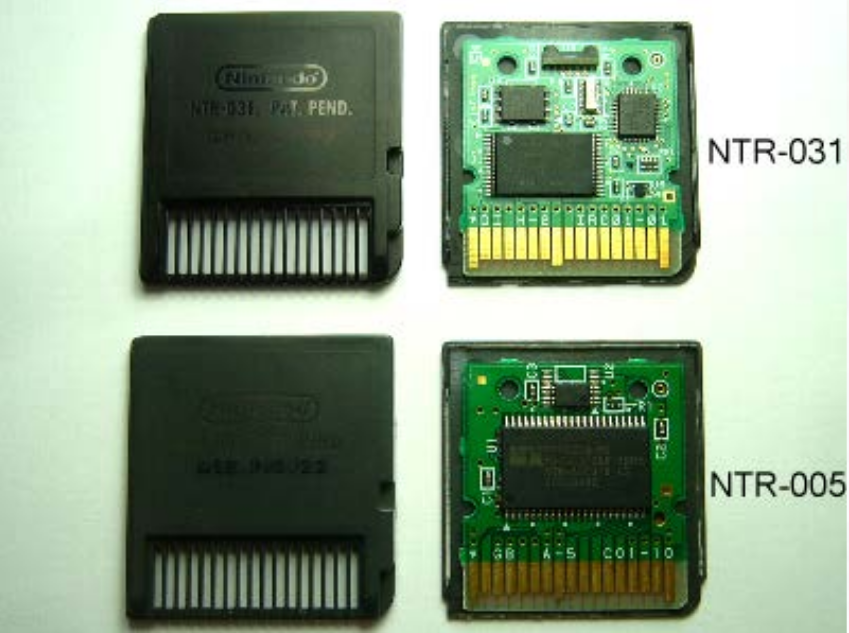
\includegraphics[width=0.5\textwidth]{archivos/gamecard.png}
  \caption{Interior de un cartucho de juego para NDS. El superior (NTR-031) añade el sensor infrarrojo.}
\textbf{Fuente:} \href{http://meseec.ce.rit.edu/551-projects/fall2015/3-1.pdf}{Thomas Farrell y Connor Petilli}
  \label{fig:gamecard}
\end{figure}














